\documentclass{article}
\title{Informe}
\usepackage[spanish]{babel}
\usepackage[utf8]{inputenc}
\usepackage{algorithm}
\usepackage{algorithmic}
\usepackage{graphicx}
\usepackage{}
\author{David Díaz Jiménez, Andrés Rojas Ortega}

\begin{document}
	
	\begin{figure}[t]
		\centering
		
\includegraphics[scale=0.2]{img/np_UJA_generica_6.png}
		
\includegraphics[scale=0.35]{img/Logo_EPS.png}
		
	\end{figure}
	
	\begin{center}
		
		\begin{large}
			
			Metaheurísticas
			
		\end{large}
		
		\vspace*{0.2in}
		\textbf{\large Informe de prácticas}
		
		\vspace*{.2in}
		
		David Díaz Jiménez, Andrés Rojas Ortega
		
		\vspace*{2.5cm}
		
	\end{center}

	\tableofcontents
	
	\newpage
	
	\section{Definición y análisis del problema}
	
	\paragraph{}Dado un conjunto \emph{N} de tamaño \emph{n}, se pide encontrar un subconjunto \emph{M} de tamaño \emph{m}, que maximice
	la función: 
	
	\[ d(s_i,M)=\sum_{s_j \in M} d(s_i,s_j)\]
	donde  $d(s_i,s_j)$ es la diversidad del elemento $s_i$ respecto al elemento $s_j$
	
	\subsection{Representación de la solución}
	
	\paragraph{} Para representar la solución se ha optado por el uso de un vector de enteros, en el que él elemento contenido en cada posición se corresponde con un integrante de la solución. La solución vendrá dada por las siguientes restricciones:
		\begin{itemize}
			
			\item La solución no puede contener elementos repetidos.
			
			\item Debe tener exactamente \emph{m} elementos.
			
			\item El orden de los elementos es irrelevante.
			
		\end{itemize}
	
	
	\subsection{Función objetivo}
	
	\[ d(s_i,M)=\sum_{s_j \in M} d(s_i,s_j)\]
	
	\subsection{Operadores comunes}
	
	\paragraph{}El operador de intercambio es el 2-opt, se seleccionara un elemento de la solución actual en base a un criterio y se sustituirá por un elemento que no pertenece a la solución. 
	
	\section{Pseudocódigo}
	
	\subsection{Greedy}
	
		\paragraph{}A continuación se procede a explicar el funcionamiento del código principal y, seguidamente, las diferentes funciones empleadas dentro del mismo.
	
	\subsubsection{Algoritmo principal}
		\begin{algorithm}[H]
			\caption{Algoritmo Greedy}
			\begin{algorithmic}
				\STATE $solucion \leftarrow GeneraSolucionInicial(semilla)$
				\STATE $candidatos \leftarrow GeneraCandidatos()$
				\WHILE{! SolucionEncontrada()}
				\STATE $candidato \leftarrow Seleccion(candidatos)$
				\IF{Factible(candidato)}
				\STATE $solucion \leftarrow solucion \cup \{candidato\}$
				\STATE $sumaResultado \leftarrow sumaResultado + Coste(candidato)$
				\ENDIF
				\STATE $candidatos \leftarrow candidatos - \{ candidato \}$
				\ENDWHILE
			\end{algorithmic}
		\end{algorithm}
	
		\paragraph{}Lo primero que realizamos es inicializar la solución con un primer elemento elegido aleatoriamente con la función "GeneraSolucionInicial(semilla)"
		
		\paragraph{}A continuación, creamos un conjunto con todos los candidatos posibles del problema, a excepción del elemento anteriormente introducido en la solución inicial. Esta tarea la realiza la función "GeneraCandidatos()".
		
		\paragraph{}Una vez realizado esto, iniciamos un bucle while - do, del cual no saldremos hasta que no hayamos encontrado una solución válida. Esta comprobación se realiza con la función "SoluciónEncontrada()".
		
		\paragraph{}El primer paso que se realiza dentro del bucle es elegir un candidato con la función "Seleccion(candidatos).
		
		\paragraph{}Una vez seleccionado un candidato, se procede a evaluar con la función "Factible(candidato) y, si resulta ser un candidato prometedor, se incluye en el conjunto solución y se actualiza el coste total de la solución acumulado.
		
		\paragraph{}El último paso a realizar en el bucle while - do es eliminar el candidato seleccionado del conjunto de candidatos, ya que ha sido evaluado (independientemente de que se haya incluido en la solución o no).
	
	

	\subsubsection{Generador de la solución inicial}
		\begin{algorithm}[H]
			\caption{GeneraSolucionInicial(semilla)}
			\begin{algorithmic}
				\STATE $solucion \leftarrow \emptyset$
				\STATE $solucionInicial \leftarrow GeneraEnteroAlearorio(semilla)$
				\STATE $solucion \leftarrow solucion \cup \{solucionInicial\}$
				\RETURN solucion
			\end{algorithmic}
		\end{algorithm}
	
		\paragraph{}El primer paso es inicializar un conjunto vacío como solución.
			
		\paragraph{}Acto seguido, se selecciona un entero aleatorio (dentro del rango de número de elementos del problema a resolver) con la función "GeneraEnteroAleatorio(semilla)". Este entero se almacena en la variable "solucionInicial".
		
		\paragraph{}Para finalizar, se incluye "solucionInicial" en la solucion vacía y se devuelve como solucion inicial.

	\subsubsection{Generador del conjunto de candidatos}
	\begin{algorithm}[H]
		\caption{GeneraCandidatos()}
		\begin{algorithmic}
			\STATE $candidatos \leftarrow \emptyset$
			\FORALL {$elemento \in matrizDatos$}
			\IF {$elemento \notin solucion$}
			\STATE $candidatos \leftarrow candidatos \cup \{elemento\}$
			\ENDIF
			\ENDFOR
			\RETURN candidatos
		\end{algorithmic}
	\end{algorithm}

	\paragraph{}El primer paso es inicializar un conjunto de candidatos vacío, llamado "candidatos".
	
	\paragraph{}A continuación, comprobamos si cada elemento de "matrizDatos" pertenece o no a la solución actual. "matrizDatos" contiene todos los elementos del problema.
	
	\paragraph{}Si pertenece a la solución actual no hacemos nada. Si no, añadimos el elemento al conjunto de candidatos "candidatos".
	
	\paragraph{}Cuando el algoritmo haya terminado de realizar todas las comprobaciones, se devuelve el conjunto de candidatos generado.

	\subsubsection{Función solución}
	\begin{algorithm}[H]
		\caption{SolucionEncontrada()}
		\begin{algorithmic}	
			\RETURN tamañoSolucion $<$ tamañoSolucionObjetivo 
		\end{algorithmic}
	\end{algorithm}

		\paragraph{}El funcionamiento de esta función resulta trivial. Simplemente devuelve si el tamaño de la solución actual es menor que el tamaño que debe tener una solución para ser aceptada o no.

	\subsubsection{Función selección}
	\begin{algorithm}[H]
		\caption{Seleccion(candidatos)}
		\begin{algorithmic}
			\STATE $max \leftarrow 0$
			\STATE $seleccionado \leftarrow \emptyset$
			\FORALL {$candidato \in candidatos$}
			\IF {Coste(candidato)$>$max}
			\STATE $max \leftarrow Coste(candidato)$
			\STATE $seleccionado \leftarrow candidato$ 
			\ENDIF
			\ENDFOR
			\RETURN seleccionado
		\end{algorithmic}
	\end{algorithm}

	\paragraph{}La variable "max" almacenará el mayor coste que aporta el mejor candidato. Inicialmente se le asigna el valor 0.
	
	\paragraph{}La variable "seleccionado" almacenará el candidato seleccionado, que es aquel que aporta un mayor coste añadiéndolo a la solución actual. Inicialmente se le asigna un valor nulo.
	
	\paragraph{}Para cada candidato del conjunto de candidatos se realiza la siguiente comprobación:
	
	\paragraph{}Se calcula el coste que aportaría a la solución si fuera incluido a esta. Si este coste calculado es mayor que la variables "max", se modifica el valor de "max" con el coste calculado y "seleccionado" se sobrescribe con el candidato evaluado.
	
	\paragraph{}Una vez realizadas todas las iteraciones del bucle for, se devuelve el candidato seleccionado.
	
	\subparagraph{Nota}En la implementación de nuestro código hemos realizado un enfoque de programación dinámica. Todos los candidatos son almacenados en un vector de pares. Cada par está formado por el candidato y un coste. Este coste se actualiza cada vez que se ejecuta al función de selección sumándole la distancia del último elemento introducido anteriormente en la solución respecto al candidato. De esta manera no tenemos que recorrer otra vez todos los elementos de la solución calculando todas sus respectivas distancias.

	\subsubsection{Función de factibilidad}
	\begin{algorithm}[H]
		\caption{Factible(candidato)}
		\begin{algorithmic}
			\RETURN candidato != -1
		\end{algorithmic}
	\end{algorithm}

	\paragraph{}El funcionamiento de esta función resulta trivial. Comprueba que el candidato a evaluar tenga un valor válido, es decir, que sea diferente del valor -1. 
	
	\paragraph{}No comprobamos que no esté repetido en la solución ya que dentro del algoritmo principal se eliminan todos los candidatos que hayan sido evaluados y, además, el elemento inicial de la solución no se introduce en el conjunto de candidatos. 
	
	\paragraph{}Por este motivo jamás se dará la situación de que esté repetido un elemento dentro de la solución.

	
	\subsection{Búsqueda Local}
	
	\subsubsection{Algoritmo principal}
	\begin{algorithm}[H]
		\caption{Busqueda local}
		\begin{algorithmic}
			\STATE GeneraSolucionInicial(semilla)
			\STATE $costeActual \leftarrow CalcularCoste()$
			\STATE $elementoMenor \leftarrow \emptyset$
			\STATE $costeSolucion \leftarrow 0$
			\STATE $mejora \leftarrow true$
			\WHILE {mejora}
			\STATE $mejora \leftarrow false$
			\STATE CalcularAportes()
			\STATE $elementoMenor \leftarrow ElementoMenorAporte()$
			\FORALL {($elemento \in matrizDatos$) $\wedge$  !(mejora)}
			\IF {!($elemento \in solucion$)}
			\STATE $mejora \leftarrow EvaluarSolucion(elemento, costeSolucion, elementoMenor)$
			\ENDIF
			\ENDFOR
			\STATE $listaAportes \leftarrow \emptyset$
			\ENDWHILE
		\end{algorithmic}
	\end{algorithm}

	\paragraph{} La primera tarea que realiza el algoritmo es generar una solución de partida. Esta solución es generada de manera aleatoria con la función "GeneraSoluciónInicial(semilla)", haciendo uso de la semilla que forma parte de los parámetros del problema.
	
	\paragraph{}Una vez generada la solución inicial, se calcula su coste con la función "CalcularCoste()". El resultado calculado se almacena en la variable "costeActual".
	
	\paragraph{}Antes de entrar en el bucle while se inicializan tres variables que serán empleadas durante el algoritmo. "elementoMenor" almacenará el elemento de la solución que aporta menos valor al coste total de la solución, se inicializa vacío. "costeSolucion" almacenará el coste de las soluciones vecinas que se vayan generando durante el transcurso de la ejecución del algoritmo, se inicializa a 0. "mejora" almacena un valor booleano e indica si el coste de la solución vecina mejora el coste de la solución global.
	
	\paragraph{}Entramos en la ejecución del bucle while. Siempre que haya mejora se ejecutan las instrucciones que se describen a continuación.
	
	\paragraph{}Primero se modifica el valor de mejora a "false". Una vez hecho esto, se calcula el valor al coste global de la solución cada uno de los elementos pertenecientes a la solución con la función "CalcularAportes()". A continuación, se extrae el elemento que menos valor aporta con la función "ElementoMenorAporte()" y se almacena en la variable "elementoMenor".
	
	\paragraph{}Entramos ahora en un bucle for que recorre cada uno de los elementos del problema, que se encuentran en "matrizDatos" siempre que el valor de mejora sea false.
	
	\paragraph{}Dentro de este bucle se comprueba que cada uno de los elementos no pertenezca a la solución. Si se da este caso, se permuta ese elemento con "elementoMenor" y se evalua si al hacer este cambia logramos una mejora del coste con la función "EvaluarSolucion(elemento,costeSolucion,elementoMenor)".
	
	\paragraph{}Una vez hecho esto, se termina el bucle for, y se modifica el valor de "listaAportes" a vacío. "listaAportes" almacena el cálculo que realiza la función "CalcularAportes()", anteriormente utilizada.

	\subsubsection{Generador de la solución inicial}
	\begin{algorithm}[H]
		\caption{GeneraSolucionInicial(semilla)}
		\begin{algorithmic}
			\WHILE{tamañoSolucion $<$ tamañoSolucionObjetivo}
			\STATE $candidato \leftarrow GeneraEnteroAleatorio(semilla)$
			\IF{$candidato \notin solucion$}
			\STATE $solucion \leftarrow solucion \cup \{candidato\}$
			\ENDIF
			\ENDWHILE
		\end{algorithmic}
	\end{algorithm}

	\paragraph{}Este algoritmo va añadiendo a la solución un elemento aleatorio, generado con la función "GeneraEnteroAleatorio(semilla)", siempre que este no forme parte ya de la solución. Esto lo realizará simpre que el número de elementos introducidos sea inferior al número de elementos que debe contener una solución para poder ser considerada como tal.

	\subsubsection{Calculo de los aportes}
	\begin{algorithm}[H]
		\caption{CalcularAportes()}
		\begin{algorithmic}
			\STATE $aporte \leftarrow 0$
			\FOR {i $<$ tamañoSolucion}
			\FOR{j $<$ tamañoSolucion}
			\STATE $aporte \leftarrow aporte + matrizDistancias[i][j]$
			\ENDFOR
			\STATE AñadirAporte(i,aporte)
			\ENDFOR
			\STATE Sort(listaAportes)
			
		\end{algorithmic}
	\end{algorithm}

	\paragraph{}Este algoritmo utiliza un doble bucle for para poder calcular la distancia total de cada elemento de la solución respecto al resto de elementos.
	
	\paragraph{}Lo primero que se realiza es inicializar la variable "aporte" a 0. Esta variable almacena el coste de cada elemento.
	
	\paragraph{}Entramos en el doble bucle que antes mencionamos y dentro de este bucle se van sumando todas las distancias para el elemento i respecto al resto de los elementos j siempre que no sean el mismo elemento.
	
	\paragraph{}Una vez termina el segundo bucle for, se almacena el coste calculado para el elemento i en la variables "listaAportes" utilizando la funcion "AñadirAporte(i,aporte)"
	
	\paragraph{}Una vez hemos realizado todos los cálculos, ordenamos "listaAportes" de menor a mayor con la función "Sort(listaAportes)" y se termina la ejecución de la función.

	\subsubsection{Calculo del elemento de la solución con menor aporte}
	\begin{algorithm}[H]
		\caption{ElementoMenorAporte()}
		\begin{algorithmic}
			\STATE $elementoMenor \leftarrow -1$
			\FORALL{$elemento \in listaAportes$}
			\IF{$elemento \notin elementosNoMejoran$}
			\STATE $elementoMenor \leftarrow elemento$
			\RETURN elementoMenor
			\ENDIF
			\ENDFOR
			\RETURN elementoMenor
		\end{algorithmic}
	\end{algorithm}

	\paragraph{}Empezamos con un bucle for que recorre todos los elementos de listaAportes.
	
	\paragraph{}Para cada elemento de listaAportes, se comprueba que este no pertenezca a la variable "elementosNoMejoran", que almacena todos los elementos que no aportan mejoran a la solución actual. Si no pertenece a esta variable, se almacena este elemento en la variable "elementoMenor" y se devuelve elementoMenor.
	
	\paragraph{}En caso de que no se haya encontrado ningún elemento que no pertenezca a "elementosNoMejoran", se devuelve "elementoMenor" con el valor comodín -1, que indica que no se ha encontrado ningún elemento válido.

	\subsubsection{Evaluación de la solución}
	\begin{algorithm}[H]
		\caption{EvaluarSolucion(elemento, costeSolucion, elementoMenor)}
		\begin{algorithmic}
			\STATE $mejora \leftarrow false$
			\STATE $costeSolucion \leftarrow CosteFactorizado(elementoMenor, elemento)$
			\IF{costeActual $<$ costeSolucion}
			\STATE Intercambio(elementoMenor, elemento)
			\STATE $costeActual \leftarrow costeSolucion$
			\STATE $mejora \leftarrow true$
			\STATE $elementosNoMejoran \leftarrow \emptyset$
			\ELSIF{elemento == tamañoMatriz-1}
			\STATE $elementosNoMejoran \leftarrow elementosNoMejoran \cup \{elementoMenor\}$
			\ENDIF
			\RETURN mejora
			\	
		\end{algorithmic}
	\end{algorithm}

	\paragraph{}Primero se inicializa la variable local "mejora" con el valor false.
	
	\paragraph{}A continuación, se almacena el coste de la solución vecina resultante de intercambiar "elementoMenor" con "elemento" en la variable "costeSolucion". "elementoMenor" pertenece a la solución y "elemento" no.
	
	\paragraph{}Se comprueba si "costeSolucion" es mayor que "costeActual", que es el coste de la solución actual.
	
	\paragraph{}En el caso de que sea mayor, se realiza el intercambio de los dos elementos con la función "Intercambio(elementoMenor,elemento)" y se almacena en "costeActual" el nuevo coste de la solución. Se actualiza el valor de mejora a true y se reinicia la variable "elementosNoMejoran" a vacío.
	
	\paragraph{}En el caso de que no sea mayor, se comprueba que el elemento evaluado no sea el último del problema. En este caso, se añade "elemento" a "elementosNoMejoran".
	
	\paragraph{}Para finalizar, se devuelve el valor de la variable local "mejora".
	
	\paragraph{}

	\subsubsection{Cálculo del coste factorizado}
	\begin{algorithm}[H]
		\caption{CosteFactorizado(elementoMenor, elemento)}
		\begin{algorithmic}
			\STATE $costeMenos \leftarrow 0$
			\STATE $costeMas \leftarrow 0$
			\FORALL{$elementoSolucion \in solucion$}
			\STATE $costeMenos \leftarrow costeMenos + matrizDistancias[elementoSolucion][elementoMenor]$
			\IF{elementoSolucion != elementoMenor}
			\STATE $costeMas \leftarrow costeMas+matrizDistancias[elementoSolucion][elemento]$
			\ENDIF
			\ENDFOR
			\RETURN costeActual - costeMenos + costeMas	
		\end{algorithmic}
	\end{algorithm}
	
	\paragraph{}Se inicializan a 0 las variables "costeMenos" y "costeMas", que almacenarán el coste que hay que restarle y sumarle respectivamente al coste total de la solución actual.
	
	\paragraph{}Una vez hecho esto, se empieza un bucle for que recorre todos los elementos de la solucion.
	
	\paragraph{}dentro del bucle se suma a "costeMenor" la distancia entre el elemento de la solucion y "elementoMenor", que es el elemento que dejará de formar parte de la solución.
	
	\paragraph{}A continuación, si el elemento de la solución no es igual que "elementoMenor", se suma a "costeMas" la distancia del elemento de la solución respecto a "elemento", que es el nuevo elemento de la solución. 
	
	\paragraph{}Una vez terminamos el bucle, se devuelve el resultado de restarle al coste de la solución actual "costeMenos" y sumarle "costeMas".
	
	\subsection{Búsqueda Tabú}
	
	
	\section{Experimentos y análisis de resultados}
	
	\subsection{Procedimiento de desarrollo de la práctica}
	
	\paragraph{}Para realizar la práctica, se ha optado por implementar lasheurísticas propuestas en el lenguaje de programación \textsc{Java}. El ejecutable que se entrega junto a este documento ha sido compilado bajo \textsc{ Apache NetBeansIDE 12.0}.
	
	\subsubsection{Equipo de pruebas}
	
	\paragraph{}Los resultados de las heurísticas han sido obtenidos en el siguiente equipo:
	
		\begin{itemize}
			
			\item Procesador: Intel Core i5 7300HQ.
			\item Memoria RAM : ?.
			\item S.O: GNU/Linux 64.
			
		\end{itemize}

	\subsubsection{Manual de usuario}
	
		\paragraph{}Para ejecutar el software asegúrese de que el archivo .jar proporcionado se ubica en el mismo directorio que la carpeta \emph{archivos}. 
		
		\paragraph{}Cunado se muestre la GUI, podrá seleccionar la heurística que desee mediante el botón correspondiente. Una vez empiece la ejecución de una heurística no sera posible seleccionar otra hasta que finalice su ejecución. Los resultados finales se mostrarán en el cuadro de texto, a su vez, se generan los log correspondientes a cada archivo y semilla en la carpeta Log, clasificados por el tipo del conjunto de datos.
	
		\begin{figure}[H]
		
			\centering
			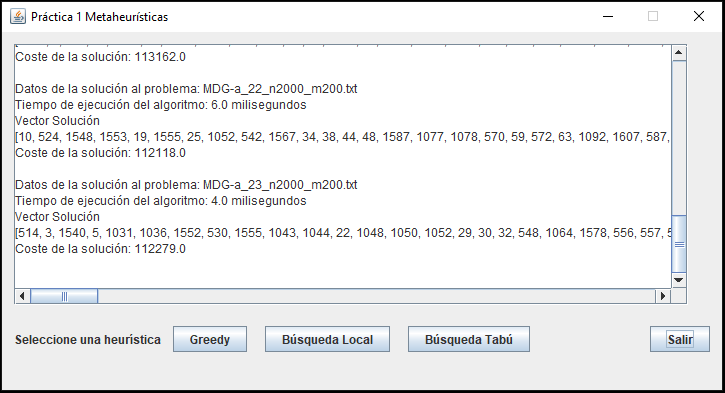
\includegraphics[scale=0.4]{img/GUI}
			\caption{GUI}
		
		\end{figure}
	
	\subsection{Parámetros de los algoritmos}
	
		\subsubsection{Greedy}
		
				\paragraph{}La heurística greedy toma como único parámetro la semilla, que se usa para generar el primer elemento de la solución, por tanto es una heurística muy cercana a un procedimiento determinista.
	
		\subsubsection{Búsqueda Local}
		
			\begin{itemize}
				
				\item Criterio de parada : Cuando no se encuentra mejora en las soluciones vecinas.
				
				\item Criterio de movimiento: Se realiza un movimiento a la primera solución vecina que nos mejore (first-improvement rule).
				
			\end{itemize}
				
	
		\subsubsection{Búsqueda Tabú}
		
			\begin{itemize}
				
				\item Iteraciones tabú: 50000.
				
				\item Memoria a corto plazo: La lista tabú tiene una tenencia de 5 elementos.
				
				\item Intentos tabú: 300, número máximo de iteraciones sin mejora antes de aplicar la oscilación estratégica.
				
				\item Memoria a largo plazo: La memoria a largo plazo se ha diseñado como un vector de enteros, la memoria no se reinicializa al realizar oscilaciones estratégicas.
				
				\item Probabilidad de reinicio: La probabilidad de reinicio a la hora de realizar la oscilación estratégica viene dada por la función :
				
				\[ \frac{nIteraciones}{maxIteraciones} \]
				
				\item Entorno de búsqueda: El numero de vecinos a evaluar en cada iteración se calcula como:
				
				\[ e^{\frac{limitIter - nIte}{ \frac{limitIter}{\log{\emph{m}}}}}\]
					
			\end{itemize}
	
	\subsubsection{Semillas}
	
	\paragraph{}Para la generación de números pseudoaleatorios se utiliza una semilla previamente definida en el archivo de configuración, en este caso es 77356084. Esta semilla se va rotando en las 5 iteraciones de cada archivo.
	
	
	\paragraph{} 77356084 $\rightarrow$ 73560847 $\rightarrow$ 35608477  ...
	
	
	\subsection{Análisis de los resultados}
	
		\subsubsection{Greedy}
		
				\paragraph{}La heurística greedy tiene un comportamiento aceptable para los conjuntos de datos escogidos, es capaz de ofrecer unos resultados cercanos a los óptimos globales mientras mantiene unos tiempos mínimos.
			
			\begin{figure}[H]
				
				\centering
				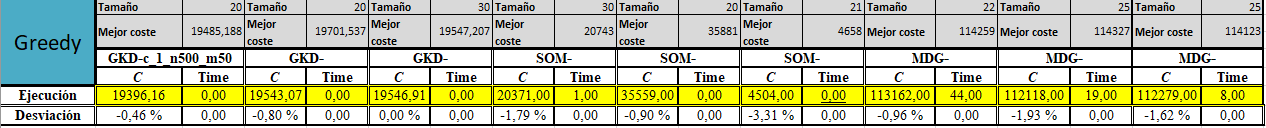
\includegraphics[scale=0.4]{img/greegyResult}
				\caption{Resultados obtenidos mediante Greedy}
				
			\end{figure}
		
		\subsubsection{Búsqueda Local}
		
				\paragraph{}Como se puede observar en la tabla de resultados, la Búsqueda Local es muy robusta en los resultados, manteniendo unos tiempos comedidos. Esto puede deberse al hecho de que es un algoritmo muy simple, no obstante, esto lo puede llevar a caer en óptimos locales.
				
			 \paragraph{}La Búsqueda local es capaz de encontrar óptimos globales en algunos casos, a diferencia de Greedy, no obstante, los tiempos pueden llegar a ser 100 veces más lentos que los obtenidos en Greedy. Debido a la eliminación de la condición de parada basada en evaluaciones, las instancias pequeñas alcanzan el optimo local en torno a las 20000 evaluaciones, mientras que las instancias más grandes necesitan unas 300000.
				
			\begin{figure}[H]
				
				\centering
				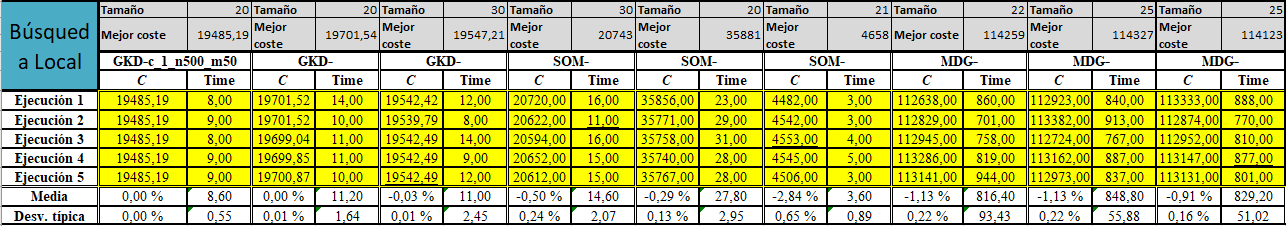
\includegraphics[scale=0.4]{img/blocalResult}
				\caption{Resultados obtenidos mediante Búsqueda Local}
				
			\end{figure}
			
		\subsubsection{Búsqueda Tabú}
	
	


	\begin{thebibliography}{0}
		
		\bibitem{Glover2020} Fred Glover, Manuel Laguna, Rafael Martí. Principles of Tabu Search. https://www.uv.es/~rmarti/paper/docs/ts1.pdf
		
		\bibitem{UgrMe2020} https://sci2s.ugr.es/graduateCourses/Metaheuristicas
		
		\bibitem{UgrAl2020}https://sci2s.ugr.es/graduateCourses/Algoritmica
		
	\end{thebibliography}

\end{document}